\documentclass[12pt]{article}
\usepackage{graphicx}
\usepackage{subfigure}

%\usepackage{geometry} % see geometry.pdf on how to lay out the page. There's lots.
%\geometry{letterpaper} % or letter or a5paper or ... etc
% \geometry{landscape} % rotated page geometry

% See the ``Article customise'' template for come common customisations

\title{Installation and Operation of the HPS SVT \\ v0.2}
\author{Timothy K. Nelson\footnote{contact person for this document}}
\date{October 19, 2014}  % delete this line to display the current date

%%% BEGIN DOCUMENT
\begin{document}

\maketitle
%\tableofcontents

\section{Description of the Silicon Vertex Tracker}
%=======================
\begin{figure}[htbp]
\begin{center}
    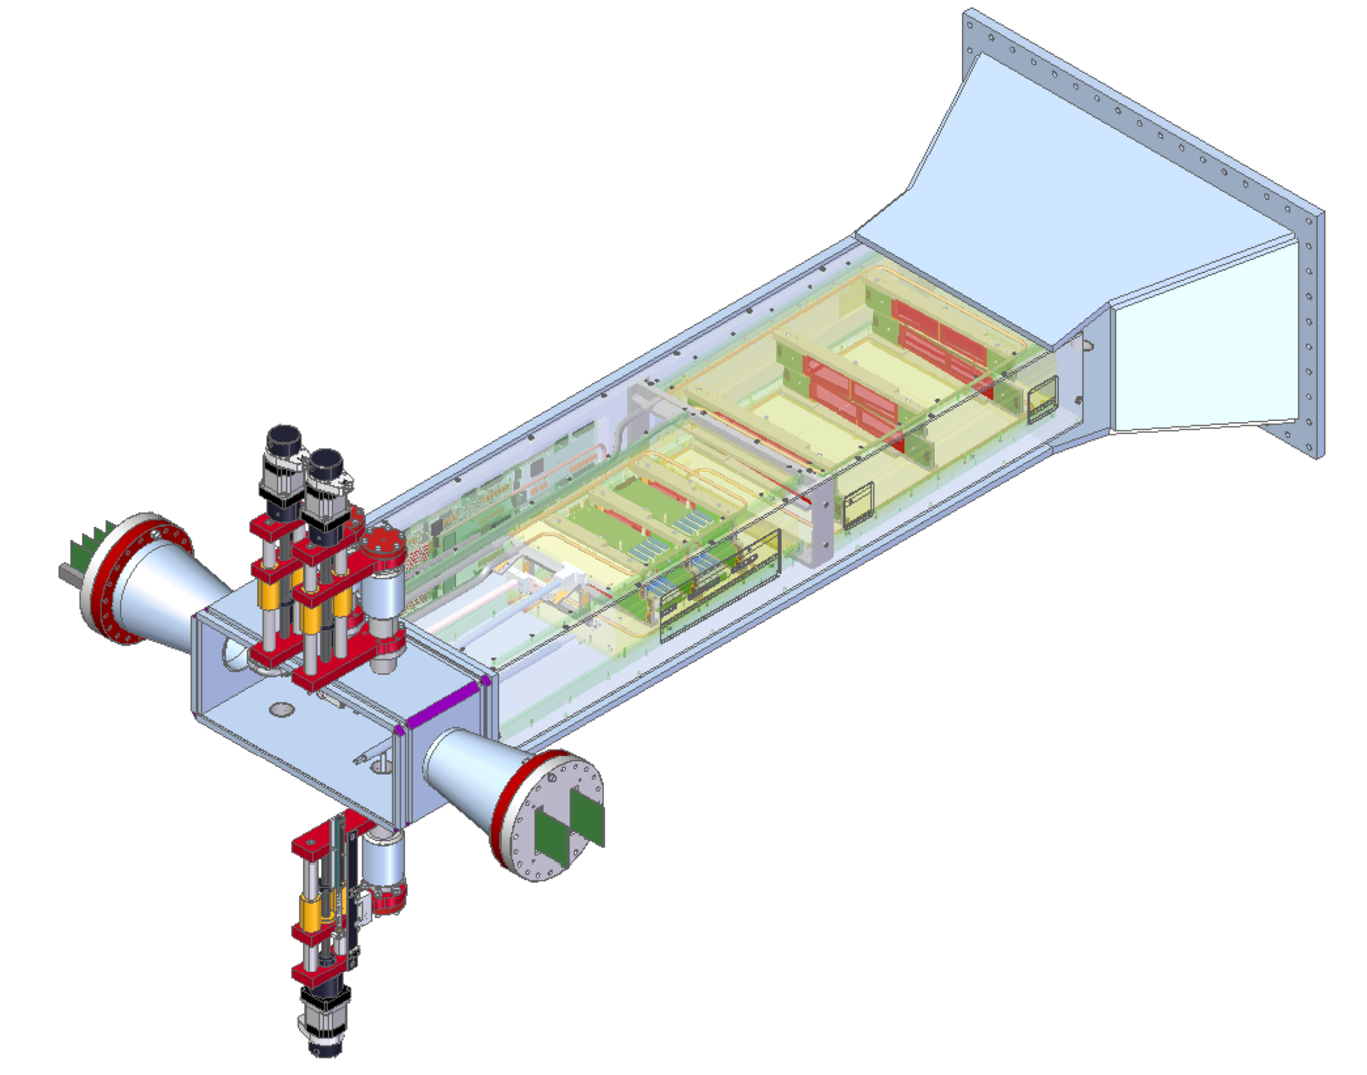
\includegraphics[width=7cm]{SVT}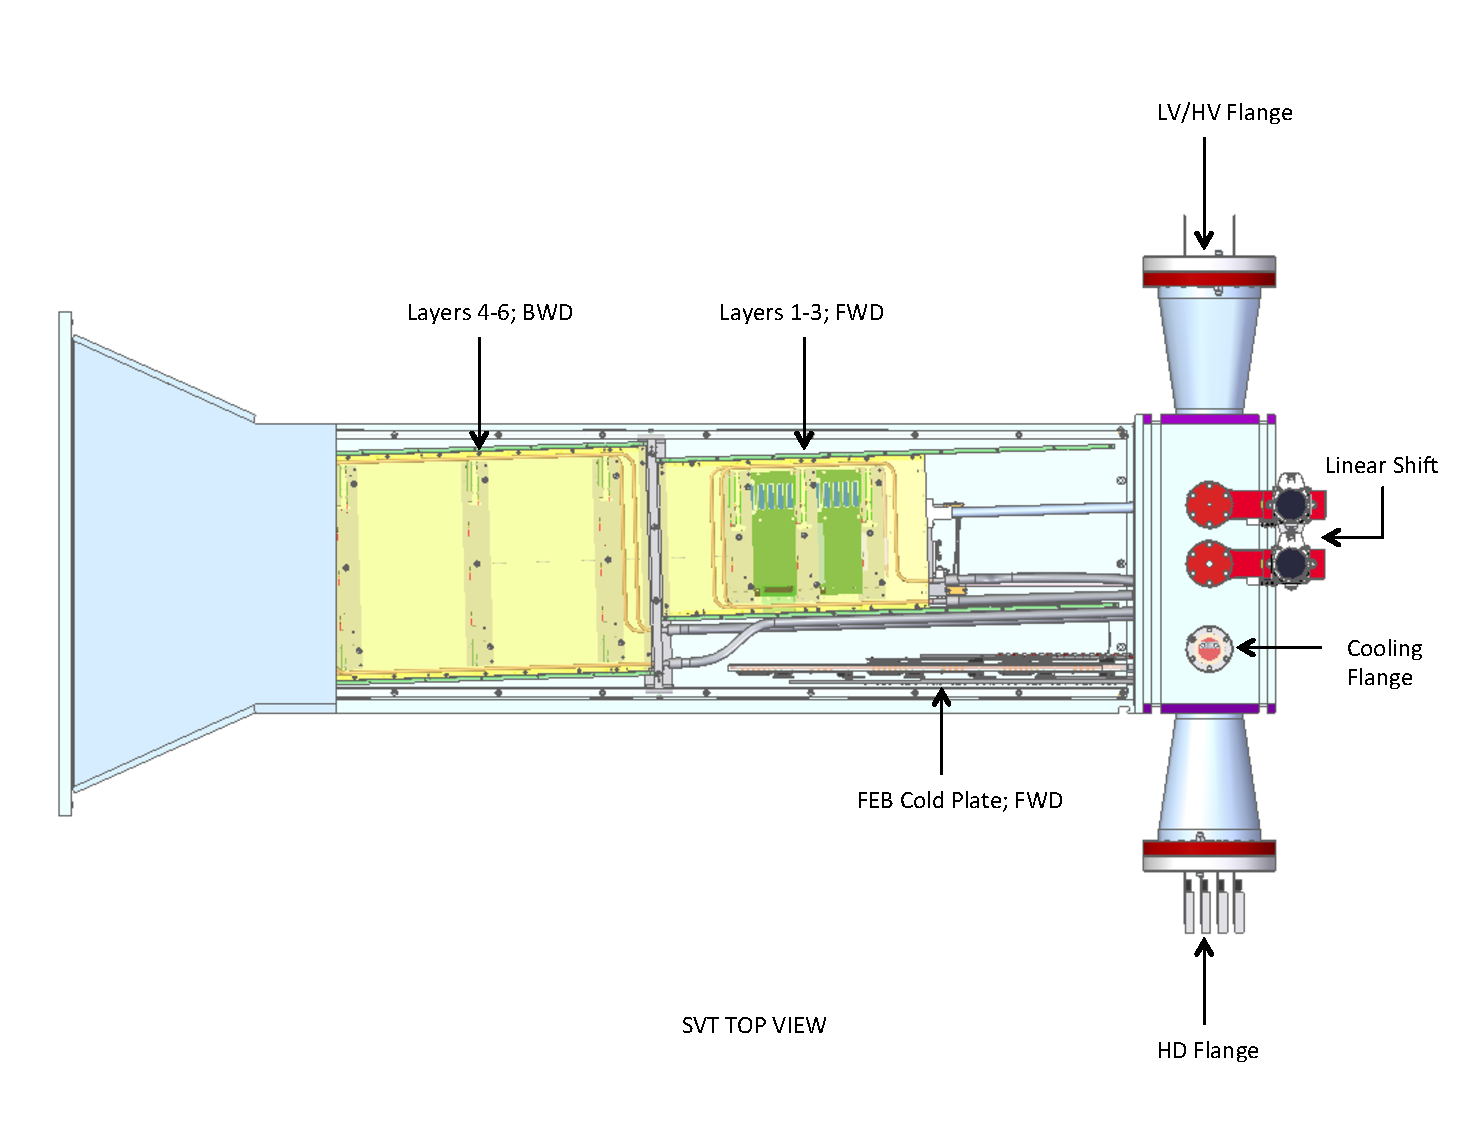
\includegraphics[width=7cm]{SVT_top}
\caption{The SVT shown inside of the pair spectrometer vacuum chamber.  The beam enters through the flange in the front of the vacuum box extension that houses services for the SVT. }
\label{fig:SVT}
\end{center}
\vspace*{-5mm}
\end{figure}
%=======================
The SVT, shown in Figure~\ref{fig:SVT}, uses 6 layers of silicon extending from 10 cm to 90 cm downstream of the target inside of the PS vacuum chamber to measure charged particle trajectories.  To accommodate the passage of the beam, the SVT is built in two halves, top and bottom, so that each layer consists of a pair of modules, one above and one below the beam plane.  Each module uses silicon microstrip sensors placed back-to-back with a small stereo angle between sides to provide 3-d space points for the hits in a module.  Modules for layer 1-3 have a single sensor on each side with readout at one end, while those for layers 4-6 are longer, with a pair of sensors on each side and readout at both ends.

Modules are supported in groups of three by a set of four support plates, as shown in Figure~\ref{fig:L1-3_bottom}. The top and bottom support plates for the back half of the SVT (layers 4-6) are stationary.  However, the supports for layers 1-3 can be opened and closed vertically around the beam, rotating around hinges behind layer 3 and moved by levers extending upstream to a pair of linear shifts outside of the magnet. The support plates are kinematically mounted inside a support box that installs into the pair spectrometer (PS) vacuum chamber, shown in Figure~\ref{fig:SVT_Box}.
%=======================
\begin{figure}[htpb]
\subfigure[\label{fig:L1-3_bottom}The lower support plate for Layers 1-3, showing the silicon (red) and readout electronics (green) of the modules, as well as the motion lever for opening and closing the SVT and the SVT beam scan wires.]
{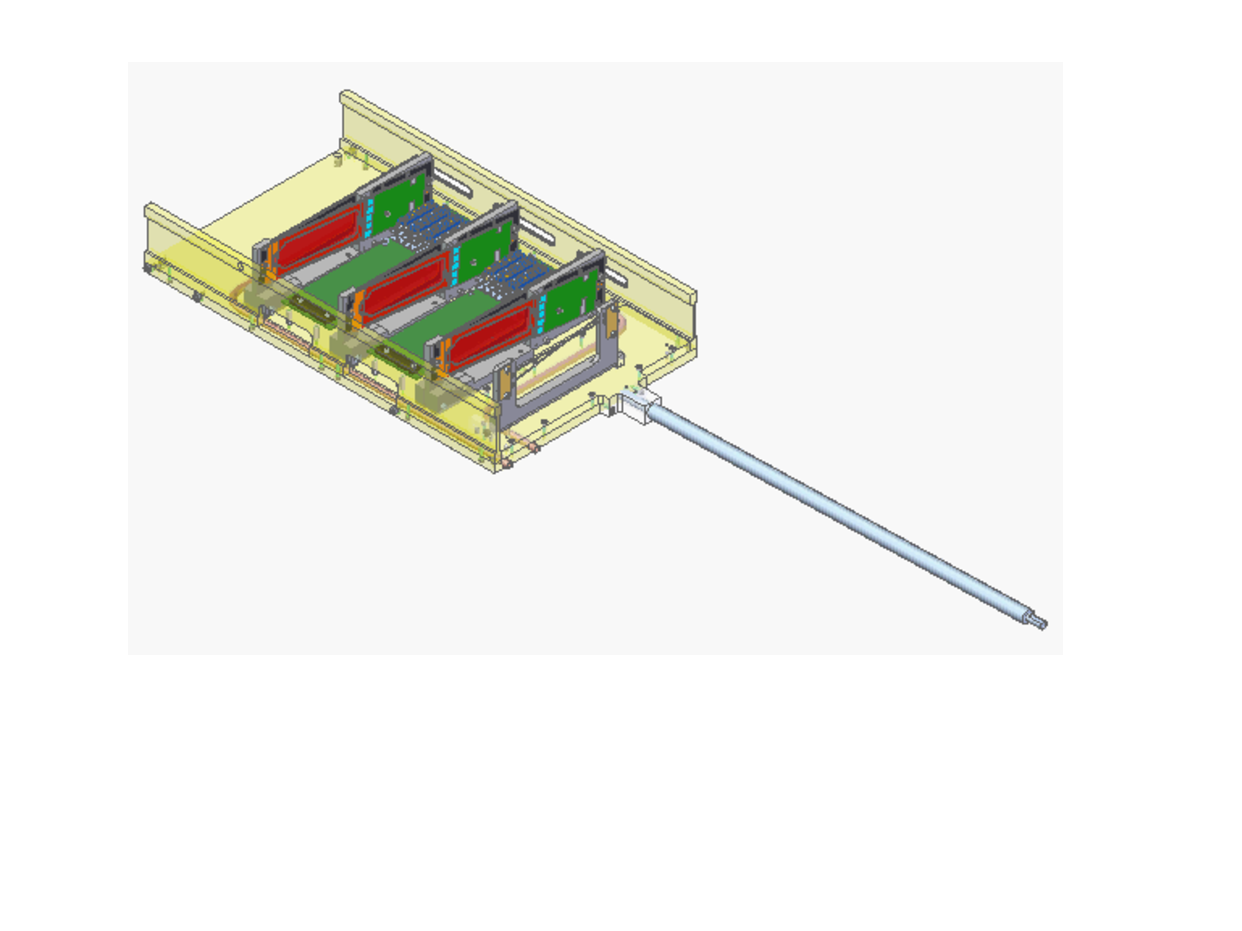
\includegraphics[width=6.5cm]{L1-3_bottom}}
\hspace{0.5cm}
\subfigure[\label{fig:SVT_Box}The SVT support box which contains the upper and lower support plates for Layers 1-3 and Layers 4-6, as well as the cooling plate housing the Front End Boards of the SVT DAQ.]
{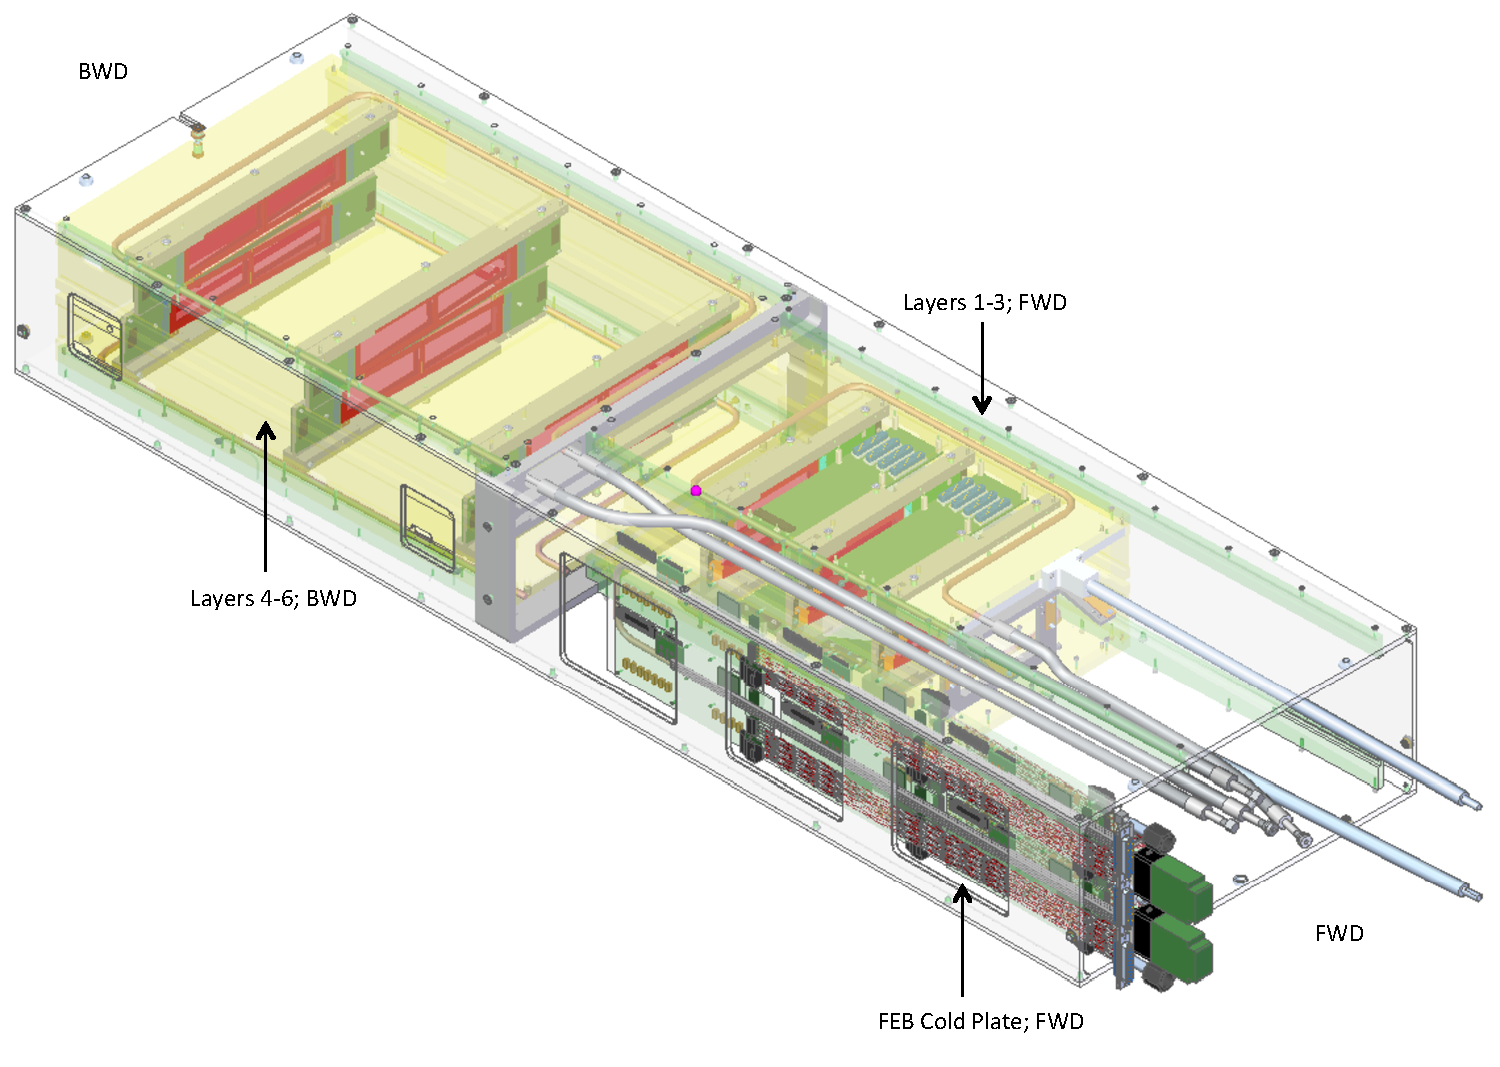
\includegraphics[width=6.5cm]{SVT_Box}}
\caption{Key sub-assemblies of the SVT.}
\end{figure}
%=======================

The first stage of readout electronics is located on a hybrid circuit board at the end of each sensor.  Multiplexed analog signals from these boards are digitized by a set of 10 Front End Boards (FEBs) mounted to a separate cooling plate inside the SVT support box. Each FEB can control 4 hybrid/sensor units: a single module in layers 4-6 and either one or two modules in layers 1-3. The FEBs also control the hybrids, provide regulated low-voltage power from a single input, and pass externally generated bias voltages (HV) through to the sensors.   The FEBs communicate with a set of 4 Signal Flange Boards (SFB), up to three per SFB, which transmit digital signals through the vacuum penetration.  The exterior side of each flange board converts digital to optical signals for communication with the RCE DAQ.  Power to the FEB are routed through a pair of Power Flange Boards, one for LV and one for HV, supplied by a Wiener Mpod power supply modules in a crate on the pie-tower.

Cooling for the SVT is provided by a pair of chillers; one for the hybrids and sensors that operates at -10 $^\circ$C and one for the FEBs that operates at room temperature.  The FEBs have a single cooling loop, while the hybrids and sensors have two loops, one for the top and one for the bottom half of the SVT, where each of these loops runs first through the support structure for layers 1-3 and then through the structure for layers 4-6.  There are temperature sensors on every hybrid as well as sensors in the FEBs.

The linear shifts, the cooling penetrations, and the signal/power penetrations are all located on a set of flanges on an extension vacuum box mounted to the upstream end of the PS vacuum chamber and which connects to the upstream beam line.

\section{SVT Installation into the Pair Spectrometer Vacuum Chamber}
This installation will require bleeding the vacuum in the region from the upstream collimator to the next valve downstream of the PS. The beam pipe between the PS and the upstream Frascati magnet must be removed, and the Frascati magnet be moved upstream.  The steps to be undertaken are:
\begin{enumerate}
\item Move SVT to Hall B (HPS \& Hall-B engineering)
\item Bleed vacuum, remove upstream beam pipe and move the Frascati magnet upstream (Hall-B engineering)
\item Move ECal downstream and remove the ECal vacuum chamber (HPS)
\item Remove the front flange from the PS vacuum chamber (Hall-B engineering)
\item Setup a table at the upstream end of the PS magnet (Hall-B engineering)
\item Place SVT on the table and insert into vacuum chamber from upstream (Hall-B engineering)
\item Survey and align SVT at upstream and downstream (survey group)
\item Install upstream vacuum box and SVT services (HPS)
\item Connect and test SVT (HPS)
\item Close vacuum chamber and pump down (Hall-B engineering)
\end{enumerate}

\section{Operation of the SVT}
Due to the proximity of the sensors to the beam, some care is required in SVT operation, especially during the process of commissioning with beam.  However, a number of systems mitigate the risk of damaging the SVT.  These include beam position scanning both upstream of and integrated in the SVT, a fast shutdown system capable of dropping the beam within 40 microseconds, and a collimator that diffuses the flux of an errant beam so that acute damage to the silicon is impossible before beam shutdown can take place.  The thickness of the collimator has been chosen based upon the results of beam damage tests with prototype modules at the SLAC NLCTA.  The steps to be taken to commission and operate the SVT with beam are described in the HPS operations manuals.

\section{SVT Cooling System}
The SVT cooling system uses a pair of chillers.  The first is Julabo Model Presto A80 operating at -30 $^\circ$C with HFE-7000 using Hall B house water for heat exchange.  The second operates at 20 $^\circ$C with water-glycol mix. The cooling pipes in vacuum are flexible metal hoses from the vacuum feed through to the detector, while the cooling lines built in the detector are 0.25� rigid copper pipe. The flexible lines are brazed on one end to the rigid copper pipes of the detectors and connected with Swagelok VCR fittings to the vacuum feedthroughs on the other end. Relief valves outside the vacuum chamber on both the supply and return lines will prevent operation above design pressure. A check valve is at the end of the main return line, just before the bypass.  The cooling system to be placed inside the vacuum chamber will be pressure tested beyond design pressure and the entire system will be operated in the lab prior to installation. All tubes and hoses exterior the the vacuum chamber will be insulated to prevent condensation.

The cooling system will automatically shut the chillers off in the event of cooling loss due to a break or obstruction in the line or loss of vacuum in the beam enclosure. The chiller will be interlocked to a flow meter installed on outlet after the tee. The same interlock signal will close a solenoid valve on the incoming line. Loss of cooling capacity or vacuum will also initiate shut down of all voltages going to SVT.  Temperature monitoring throughout the SVT prevents detector operation without adequate cooling.

\section{SVT Materials}

Every component of the SVT was tested for vacuum and magnet compatibility. In addition, nearly all of the components are being re-used from HPS test or are fabricated from the exact same materials from the same vendors and using the same techniques.  There are a small number new materials, listed in Table~\ref{tab:materials}.  
%===================
\begin{table}[ht]
\begin{center}
\begin{tabular}{llc}   
\hline \hline 
    Component & Material & Inside Vacuum? \\      
\hline
%\multicolumn{4}{l}{b} \\
structural epoxy & Hysol 9396 & Y  \\
conductive epoxy & Epoxies Inc. 40-3905 & Y \\
magnet wire insulation & polyester-imide & Y \\ 
HV Connectors & & Y \\
high-speed data cables & & Y \\
high-speed data connectors & stainless steel & Y \\
cooling feed-throughs & aluminum oxide ceramic & Y \\
bearings & aluminum oxide ceramic & Y \\
kinematic mounts & tungsten carbide & Y \\
L4-6 adjustment screw & phosphor bronze & Y \\
Optical transceivers & & N \\ 
 \hline \hline
\end{tabular}
\caption[]{The proposed layout of the HPS SVT.}
\label{tab:materials} 
\end{center}
\end{table}
%===================
These have all been tested at SLAC to $10^{-6}$ Torr using the same methodology as for HPS Test.  In addition, a new process for vacuum penetration of the Flange Boards was developed at SLAC. These flanges have passed a helium vacuum leak check at SLAC. The vacuum box with all flanges will be tested and pumped down to $10^{-6}$ Torr at SLAC before shipping to JLab. Non-magnetic materials are used since the SVT operates in a magnetic field.  

Known radiation tolerant materials and devices are used in the SVT modules, and shielding protects the the FEBs facing the target from x-rays, which may reach significant levels during the useful life of the silicon.  The susceptibility of key components to neutron irradiation has been studied and compared to simulated doses, which have been found to be well below levels of concern.

The SVT will require high voltage (HV) and low voltage (LV) power. A rack with two Wiener mainframes loaded with HV and LV Mpod modules will be installed on the "pie tower" and a breakout box and patch panel for power will be mounted solidly on an aluminum frame on top of the PS magnet.

\section{SVT Positioning System}

The positioning system uses linear shifts mounted above and below the vacuum box with bellows allowing for the transfer of motion to the upper/lower SVT detectors in layers 1-3. Calibration will be performed for the placement of detectors for electron running. There are both safety stops and microswitches used to limit motion to safe ranges. In addition, the construction of the SVT supports prevents the upper and lower SVT from colliding.  The remote operation of the positioning system will be tested at SLAC, as well as at JLAB before and after installation. Correct operation of all switches and safety stops will be verified at JLAB during setup and after the detector is installed on beam line. 

The linear stage has 4 inch travel driven by an 8 wire stepper motor configured for 4 wire bipolar series connection. A Newport XPS-Q8 Motion Controller is used to drive the stepper motor and Slow Control GUI based on EPICS. The following tests were done at SLAC before shipment: Basic stepper motor function test, stage positioning accuracy measurement, leak check the bellows, and operation in magnetic field up to 300 Gauss at the motor. The stage positing accuracy is $\approx10$ $\mu$m with a directional backlash of 25 $\mu$m.  The stepper motor function was tested under vacuum load and the SVT weight.

\end{document}